\documentclass[11pt]{article}
\usepackage{listings}
\usepackage{tikz}
\usepackage{algorithm2e}
\usetikzlibrary{arrows,automata,shapes}
\tikzstyle{block} = [rectangle, draw, fill=blue!20, 
    text width=5em, text centered, rounded corners, minimum height=2em]

\newtheorem{defn}{Definition}
\newtheorem{crit}{Criterion}

\newcommand{\handout}[5]{
  \noindent
  \begin{center}
  \framebox{
    \vbox{
      \hbox to 5.78in { {\bf Software Testing, Quality Assurance and Maintenance } \hfill #2 }
      \vspace{4mm}
      \hbox to 5.78in { {\Large \hfill #5  \hfill} }
      \vspace{2mm}
      \hbox to 5.78in { {\em #3 \hfill #4} }
    }
  }
  \end{center}
  \vspace*{4mm}
}

\newcommand{\lecture}[4]{\handout{#1}{#2}{#3}{#4}{Lecture #1}}
\topmargin 0pt
\advance \topmargin by -\headheight
\advance \topmargin by -\headsep
\textheight 8.9in
\oddsidemargin 0pt
\evensidemargin \oddsidemargin
\marginparwidth 0.5in
\textwidth 6.5in

\parindent 0in
\parskip 1.5ex
%\renewcommand{\baselinestretch}{1.25}

\begin{document}

\lecture{15 --- February 6, 2015}{Winter 2015}{Patrick Lam}{version 1}
\section*{Data flow Criteria}

So far we've seen structure-based criteria which imposed test
requirements solely based on the nodes and edges of a graph. These
criteria have been oblivious to the contents of the nodes.

However, programs mostly move data around, so it makes sense to
propose some criteria based on the flow of data around a program.
We'll be talking about $du$-pairs, which connect definitions and
uses of variables.
\[
\mbox{du-pair} \left[ \begin{array}{lcl} 
\mbox{\tt x = 5} & \hspace*{2em} & \mbox{\tt // def(x)} \\
\vdots \\
\mbox{\tt print(x)} & \hspace*{2em} & \mbox{\tt // use(x)} \\
\end{array} \right.
\]

Let's look at some graphs. 
\begin{center}
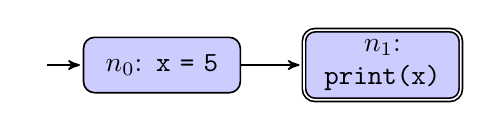
\begin{tikzpicture}[->,>=stealth',shorten >=1pt,auto,node distance=2.8cm,
                    semithick,initial text=]

  \node[initial,block]   (1)              {$n_0$: {\tt x = 5}};
  \node[accepting,block] (2) [right of=1] {$n_1$: {\tt print(x)}};
  
  \path (1) edge              node {} (2);
\end{tikzpicture}
\end{center}
{\sf We write }\\[1em]
\[ \mbox{def}(n_0) = \mbox{use}(n_1) = \{ x \}.\] 
Note that edges can also have defs and uses, for instance in a 
graph corresponding to a finite state machine. In that case, 
{\sf we could write:} \\[1em]
\[ \mbox{use}(n_0, n_1) = \{ \}.\] 

Here's another example.

\begin{center}
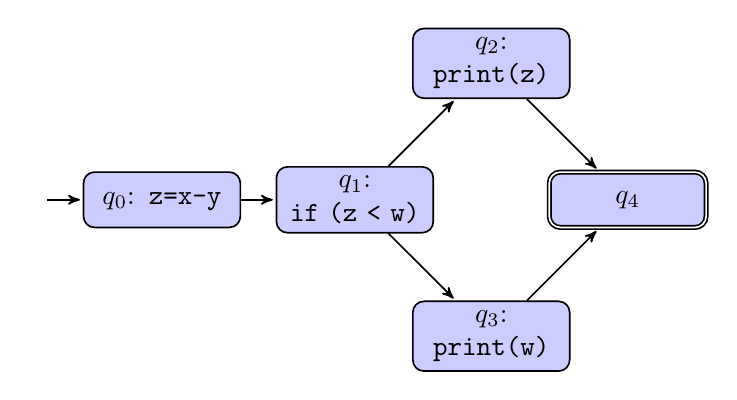
\begin{tikzpicture}[->,>=stealth',shorten >=1pt,auto,node distance=2.45cm,
                    semithick,initial text=]

  \node[initial,block]   (1)              {$q_0$: {\tt z=x-y}};
  \node[block]   (2) [right of=1]             {$q_1$: \\ {\tt if (z < w)}};
  \node[block]   (3) [above right of=2]             {$q_2$: {\tt print(z)}};
  \node[block]   (4) [below right of=2]             {$q_3$: {\tt print(w)}};
  \node[accepting,block] (5) [below right of=3] {$q_4$};
  
  \path (1) edge              node {} (2)
        (2) edge              node {} (3)
        (2) edge              node {} (4)
        (3) edge              node {} (5)
        (4) edge              node {} (5);
\end{tikzpicture}
\end{center}
% uses and defs

A particular def $d$ of variable $x$ may (or may not) \emph{reach} a
particular use $u$.  If a def may reach a particular use, then there
exists a path from $d$ to $u$ which is free of redefinitions of $x$.
In the following graph, the def at $n_2$ does not reach the use at $n_3$,
since no path goes from $n_2$ to $n_3$.

\begin{center}
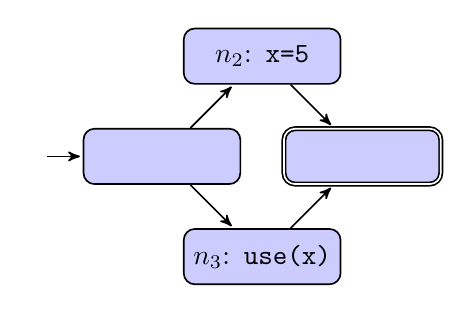
\begin{tikzpicture}[->,>=stealth',shorten >=1pt,auto,node distance=1.8cm,
                    semithick,initial text=]

  \node[initial,block]   (1)              {};
  \node[block]   (3) [above right of=1]             {$n_2$: {\tt x=5}};
  \node[block]   (4) [below right of=1]             {$n_3$: {\tt use(x)}};
  \node[accepting,block] (5) [below right of=3] {};
  
  \path (1) edge              node {} (3)
        (1) edge              node {} (4)
        (3) edge              node {} (5)
        (4) edge              node {} (5);
\end{tikzpicture}
\end{center}
Another example of a definition which does not reach:
\begin{center}
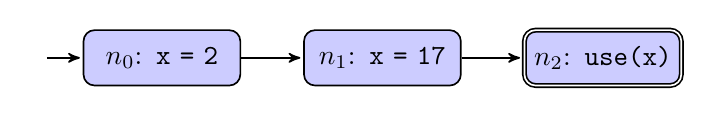
\begin{tikzpicture}[->,>=stealth',shorten >=1pt,auto,node distance=2.8cm,
                    semithick,initial text=]

  \node[initial,block]   (1)              {$n_0$: {\tt x = 2}};
  \node[block]           (2) [right of=1] {$n_1$: {\tt x = 17}};
  \node[accepting,block] (3) [right of=2] {$n_2$: {\tt use(x)}};
  
  \path (1) edge              node {} (2)
        (2) edge              node {} (3);
\end{tikzpicture}
\end{center}
We say that the definition at $n_1$ \emph{kills} the definition at
$n_0$, so that $\mbox{def}(n_0)$ does not reach $n_2$. We are therefore
looking for def-clear paths.

\begin{defn}
A path $p$ from $\ell_1$ to $\ell_m$ is \emph{def-clear} with respect
to variable $v$ if for every node $n_k$ and every edge $e_k$ on $p$
from $\ell_1$ to $\ell_m$, where $k \neq 1$ and $k \neq m$, then $v$
is not in $\mbox{def}(n_k)$ or in $\mbox{def}(e_k)$.
\end{defn}
That is, nothing on the path $p$ from location $\ell_1$ to location
$\ell_m$ redefines $v$. (Locations are edges or nodes.)
\begin{defn} 
A def of $v$ at $\ell_i$ reaches a use of $v$ at $\ell_2$ if there
exists a def-clear path from $\ell_i$ to $\ell_j$ with respect to $v$.
\end{defn}

Quick poll: does the def at $n_0$ reach the use at $n_5$?
\begin{center}
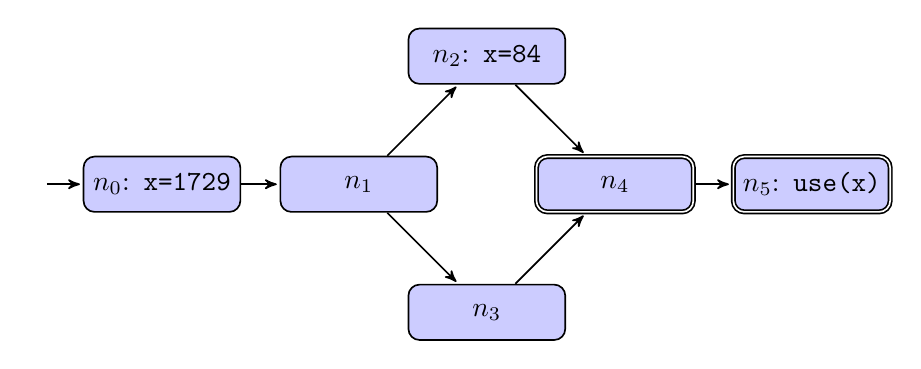
\begin{tikzpicture}[->,>=stealth',shorten >=1pt,auto,node distance=2.3cm,
                    semithick,initial text=]

  \node[initial,block]   (1)              {$n_0$: {\tt x=1729}};
  \node[block]   (2) [right of=1,xshift=0.2cm]             {$n_1$};
  \node[block]   (3) [above right of=2]             {$n_2$: {\tt x=84}};
  \node[block]   (4) [below right of=2]             {$n_3$};
  \node[accepting,block] (5) [below right of=3] {$n_4$};
  \node[accepting,block] (6) [right of=5,xshift=0.2cm] {$n_5$: {\tt use(x)}};
  
  \path (1) edge              node {} (2)
        (2) edge              node {} (3)
        (2) edge              node {} (4)
        (3) edge              node {} (5)
        (4) edge              node {} (5)
        (5) edge              node {} (6);
\end{tikzpicture}
\end{center}
Building on the notion of a def-clear path:

\begin{defn}
A \emph{du-path} with respect to $v$ is a simple path that is def-clear with
respect to $v$ from a node $n_i$, such that $v$ is in $\mbox{def}(n_i)$,
to a node $n_j$, such that $v$ is in $\mbox{use}(n_j)$.
\end{defn}

(This definition could be easily modified to use edges $e_i$ and $e_j$).

{\sf Note the following three points about \emph{du}-paths:}
\begin{itemize}
\item associated with a variable
\item simple (otherwise there are too many)
\item may be any number of uses in a du-path
\end{itemize}

\section*{Coverage criteria using \mbox{du}-paths}

We next create groups of \emph{du}-paths. Consider
again the following double-diamond graph $D$:
\begin{center}
\label{D}
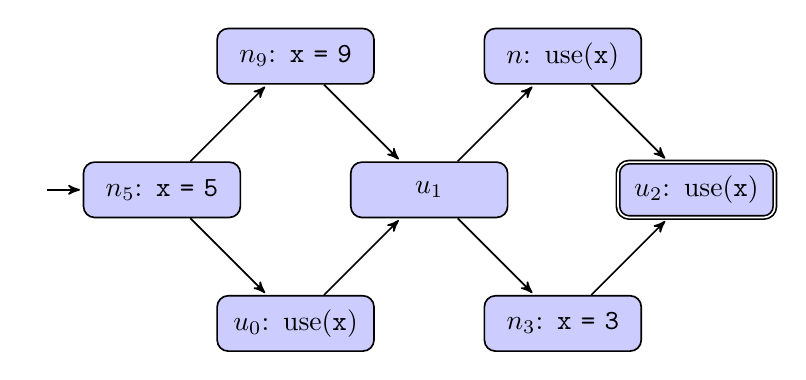
\begin{tikzpicture}[->,>=stealth',shorten >=1pt,auto,node distance=2.4cm,
                    semithick,initial text=]

  \node[initial,block]   (n5)                     {$n_5$: {\tt x = 5}};
  \node[block]           (u0) [below right of=n5] {$u_0$: use({\tt x})};
  \node[block]           (n9) [above right of=n5] {$n_9$: {\tt x = 9}};
  \node[block]           (u1) [below right of=n9] {$u_1$};
  \node[block]           (n3) [below right of=u1] {$n_3$: {\tt x = 3}};
  \node[block]           (n)  [above right of=u1] {$n$: use({\tt x})};
  \node[accepting,block] (u2) [below right of=n] {$u_2$: use({\tt x})};
  
  \path (n5) edge              node {} (u0)
             edge              node {} (n9)
        (u0) edge              node {} (u1)
        (n9) edge              node {} (u1)
        (u1) edge              node {} (n3)
             edge              node {} (n)
        (n3) edge              node {} (u2)
        (n) edge              node {} (u2);
\end{tikzpicture}
\end{center}

We will define two sets of {\em du}-paths:
\begin{itemize}
\item def-path sets: fix a def and a variable, e.g. 
\begin{itemize} 
\item $\mbox{du}(n_5, x) =$
\item $\mbox{du}(n_3, x) =$
\end{itemize}
\item def-pair sets: fix a def, a use, and a variable, 
e.g. $\mbox{du}(n_5, n, x) =$
\end{itemize}

These sets will give the notions of all-defs coverage (tour at least
one {\em du}-path from each def-path set---a weak criterion) and all-uses
coverage (tour at least one {\em du}-path from each def-pair set).
%; and all-du-paths coverage (tour all {\em du}-paths from each def-pair set).

{\sf How can there be multiple elements in a def-pair set?}
% multiple def-clear paths from $n_i$ to $n_j$.

\newpage

Here's an example with two \emph{du}-paths in a def-pair set.
\begin{center}
\label{C}
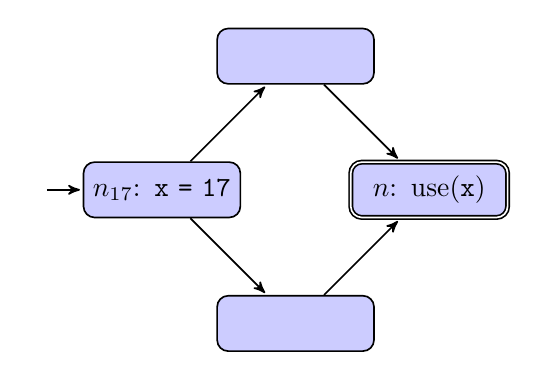
\begin{tikzpicture}[->,>=stealth',shorten >=1pt,auto,node distance=2.4cm,
                    semithick,initial text=]

  \node[initial,block]   (n17)                     {$n_{17}$: {\tt x = 17}};
  \node[block]           (u0) [below right of=n17] {};
  \node[block]           (u1) [above right of=n17] {};
  \node[accepting,block] (n) [below right of=u1] {$n$: use({\tt x})};
  
  \path (n17) edge              node {} (u0)
              edge              node {} (u1)
        (u0) edge              node {} (n)
        (u1) edge              node {} (n);
\end{tikzpicture}
\end{center}
{\sf We then have}
\[ \mbox{du}(n_{17}, n, x) = \]

Note the general relation
\[ \mbox{du}(n_i, v) = \bigcup_{n_j} \mbox{du}(n_i, n_j, v) \]
There are more def-pair sets than def-path sets. Cycles are 
always allowed as \emph{du}-paths, as long as the \emph{du}-path
is simple; you can always tour a \emph{du}-path with a non-simple
path, of course.

\paragraph{Useful exercise.} Create an example where one def-path
set splits into several def-pair sets; you can get a smaller example
than the one in the book.

%% \subsection*{Touring \emph{du}-paths}
%% \begin{defn} 
%% A test path $p$ \emph{du-tours} subpath $d$ with
%% respect to $v$ if $p$ tours $d$ and $d$ is def-clear
%% with respect to $v$.
%% \end{defn}

%% We could allow or disallow def-clear sidetrips. Def-clear sidetrips
%% make more paths tourable, so we choose to allow them.
%% The definition then says that the part of $p$ that \emph{du}-tours $d$
%% must be def-clear.

We can use the above definitions to provide coverage criteria.
\begin{crit}
{\bf All-Defs Coverage} (ADC). For each def-path set $S = \mbox{du}(n, v)$,
TR contains at least one path $d$ in $S$.
\end{crit}

\begin{crit}
{\bf All-Uses Coverage} (AUC). For each def-pair set $S = \mbox{du}(n_i, n_j,
v)$, TR contains at least one path $d$ in $S$.
\end{crit}

%% \begin{crit}
%% {\bf All-du-paths Coverage} (ADUPC). For each def-pair set 
%% $S = \mbox{du}(n_i, n_j, v)$, TR contains every path $d$ in $S$.
%% \end{crit}

\newpage
What do these criteria mean? For each def,
\begin{itemize}
\item ADC: reach at least one use;
\item AUC: reach every use somehow;
%\item ADUPC: reach every use in every simple way (all \mbox{\em du}-paths).
\end{itemize}

{\sf In the context of the earlier example,}
\begin{itemize}
\item ADC requires:
\item AUC requires:
%\item ADUPC requires: same as AUC since def-pair sets are all singletons.
\end{itemize}

\paragraph{Nodes versus edges.}
So far, we've assumed definitions and uses occur on nodes.
\begin{itemize}
\item uses on edges (``$p$-uses'') work as well;
\item defs on edges are trickier, because a \emph{du}-path from an edge
to an edge may not be simple. (We could make things work out with more work.)
\end{itemize}

\paragraph{Another example.}
\begin{center}
\label{DD}
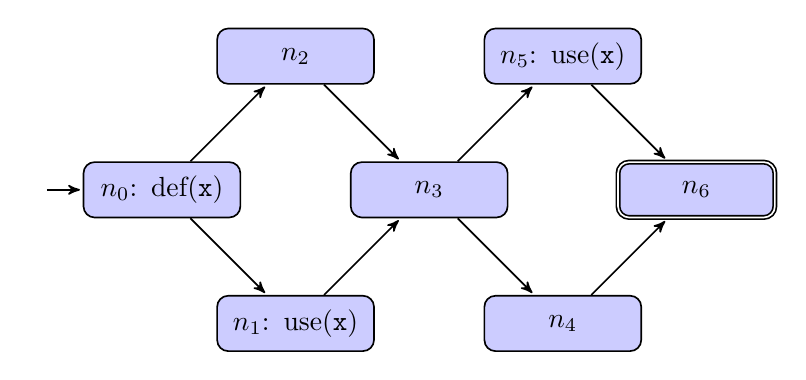
\begin{tikzpicture}[->,>=stealth',shorten >=1pt,auto,node distance=2.4cm,
                    semithick,initial text=]

  \node[initial,block]   (n0)                     {$n_0$: def({\tt x})};
  \node[block]           (n1) [below right of=n0] {$n_1$: use({\tt x})};
  \node[block]           (n2) [above right of=n0] {$n_2$};
  \node[block]           (n3) [below right of=n2] {$n_3$};
  \node[block]           (n4) [below right of=n3] {$n_4$};
  \node[block]           (n5) [above right of=n3] {$n_5$: use({\tt x})};
  \node[accepting,block] (n6) [below right of=n5] {$n_6$};
  
  \path (n0) edge              node {} (n1)
             edge              node {} (n2)
        (n1) edge              node {} (n3)
        (n2) edge              node {} (n3)
        (n3) edge              node {} (n4)
             edge              node {} (n5)
        (n5) edge              node {} (n6)
        (n4) edge              node {} (n6);
\end{tikzpicture}
\end{center}

Some test sets that meet these criteria:
\begin{itemize}
\item ADC: % 0 - 1
\item AUC: % 0 - 1; 0 - 2 - 3 - 5
%\item ADUPC: % 0 - 1; 0 - 1 - 3 - 5; 0 - 2 - 3 - 5
\end{itemize}


\end{document}
